\documentclass{beamer}

\mode<presentation>
{
  \usetheme{CambridgeUS}
  \setbeamercovered{transparent}
}

\usepackage[english]{babel}
\usepackage[latin1]{inputenc}
\usepackage{times}
\usepackage[T1]{fontenc} 
% Or whatever. Note that the encoding and the font should match. If T1
% does not look nice, try deleting the line with the fontenc.
\usepackage{amsmath}

\newcommand{\linespace}{\vskip 0.25cm}

\definecolor{MyForestGreen}{rgb}{0,0.7,0} 
\newcommand{\tableemph}[1]{{#1}}
\newcommand{\tablewin}[1]{\tableemph{#1}}
\newcommand{\tablemid}[1]{\tableemph{#1}}
\newcommand{\tablelose}[1]{\tableemph{#1}}

\definecolor{MyLightGray}{rgb}{0.6,0.6,0.6}
\newcommand{\tabletie}[1]{\color{MyLightGray} {#1}}

% The text in square brackets is the short version of your title and will be used in the
% header/footer depending on your theme.
\title[Analysis of GP Ancestry in Neo4j]{Analysis of Ancestry in Genetic Programming with a Graph Database}

% Sub-titles are optional - uncomment and edit the next line if you want one.
% \subtitle{Why does sub-tree crossover work?} 

% The text in square brackets is the short version of your name(s) and will be used in the
% header/footer depending on your theme.
\author[Donatucci, Dramdahl, McPhee]{David Donatucci \\ M. Kirbie Dramdahl \\ Nicholas Freitag McPhee}

% The text in square brackets is the short version of your institution and will be used in the
% header/footer depending on your theme.
\institute[UMM]
{
  Division of Science and Mathematics \\
  University of Minnesota, Morris \\
  Morris, Minnesota, USA
}

% The text in square brackets is the short version of the date if you need that.
\date[April '14, MICS, Verona, WI] % (optional)
{25 April 2014 \\ MICS, Verona, WI}

% Delete this, if you do not want the table of contents to pop up at
% the beginning of each subsection:
\AtBeginSection[]
{
  \begin{frame}<beamer>
    \frametitle{Outline}
    \tableofcontents[currentsection, hideothersubsections]
  \end{frame}
}

\begin{document}

\begin{frame}
  \titlepage
\end{frame}

% For a 20-25 minute senior seminar talk you probably want something like:
% - Two or three major sections (other than the summary).
% - At *most* three subsections per section.
% - Talk about 30s to 2min per frame. So there should probably be between
%   15 and 30 frames, all told.

\section*{Overview}

\subsection*{The Big Picture}

\begin{frame}
  \frametitle{The Big Picture}
  
  \begin{columns}
  \begin{column}{0.6\textwidth}
  \begin{itemize}
  	\item The power of graph databases: analyzing internal data of GP
	\item ???????????
	\item Even fewer allow for plasticity during development????
	\item N-gram GP has natural developmental phase?????
	\item Can we find useful information about runs?
  \end{itemize}
  \end{column}
  \begin{column}{0.4\textwidth}
   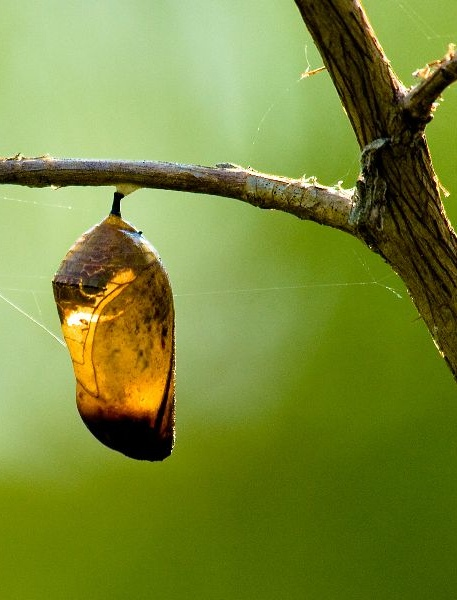
\includegraphics[width=0.95\textwidth]{Illustrations/Empty_cocoon_crop_by_Bluedrakon_from_Flickr.jpg}
       \\
    \only{\tiny{Bluedrakon \\ \url{http://tr.im/pWUi} }}
  \end{column}
  \end{columns}
\end{frame}

\subsection*{Outline}

\begin{frame}
  \frametitle{Outline}
  \tableofcontents[hideallsubsections]
\end{frame}

\section[Genetic Programming]{Genetic Programming}

\subsection{GP Overview}

\begin{frame}
  \frametitle{Genetic Programming Overview}
  
  \begin{columns}
  \begin{column}{.65\textwidth}
  \begin{itemize}
  	\item Genetic Programmings is based upon biological principles.
	\item Individuals form a population.
	\item Transformations
		\begin{itemize}
		\item Crossover (XO)
		\item Mutation
		\item Reproduction
		\item Elitism
		\end{itemize}
	\item Transformations occur over a specified amount of generations.
	\item Individuals are rated by their fitness.
  \end{itemize}
  \end{column}
  \begin{column}{.35\textwidth}
    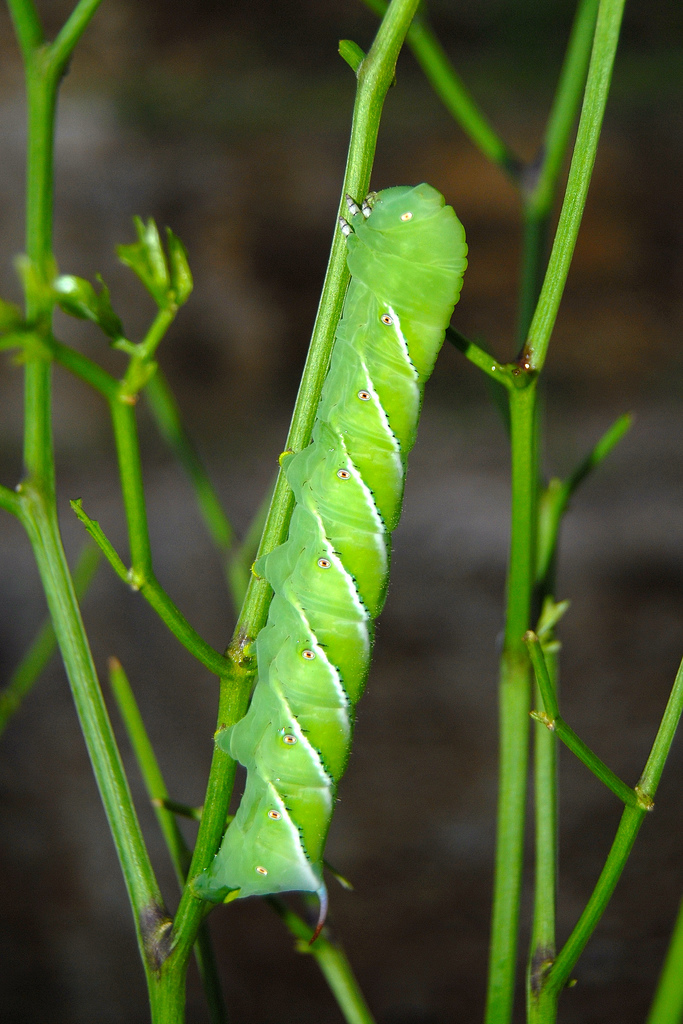
\includegraphics[width=.95\textwidth]{Illustrations/Manduca_sexta_by_Sam_Fraser-Smith_from_Flickr.jpg}
    \\
    \tiny{Sam Fraser-Smith \\ \url{http://tr.im/pq7l} }
  \end{column}
  \end{columns}

\end{frame}

\begin{frame}
  \frametitle{Transformations}

		\begin{itemize}
		\item[Crossover (XO)] sexual reproduction (root and non-root)
		\item[Mutation] subtrees altered
		\item[Reproduction] asexual reproduction
		\item[Elitism] reproduction based on fitness
		\end{itemize}
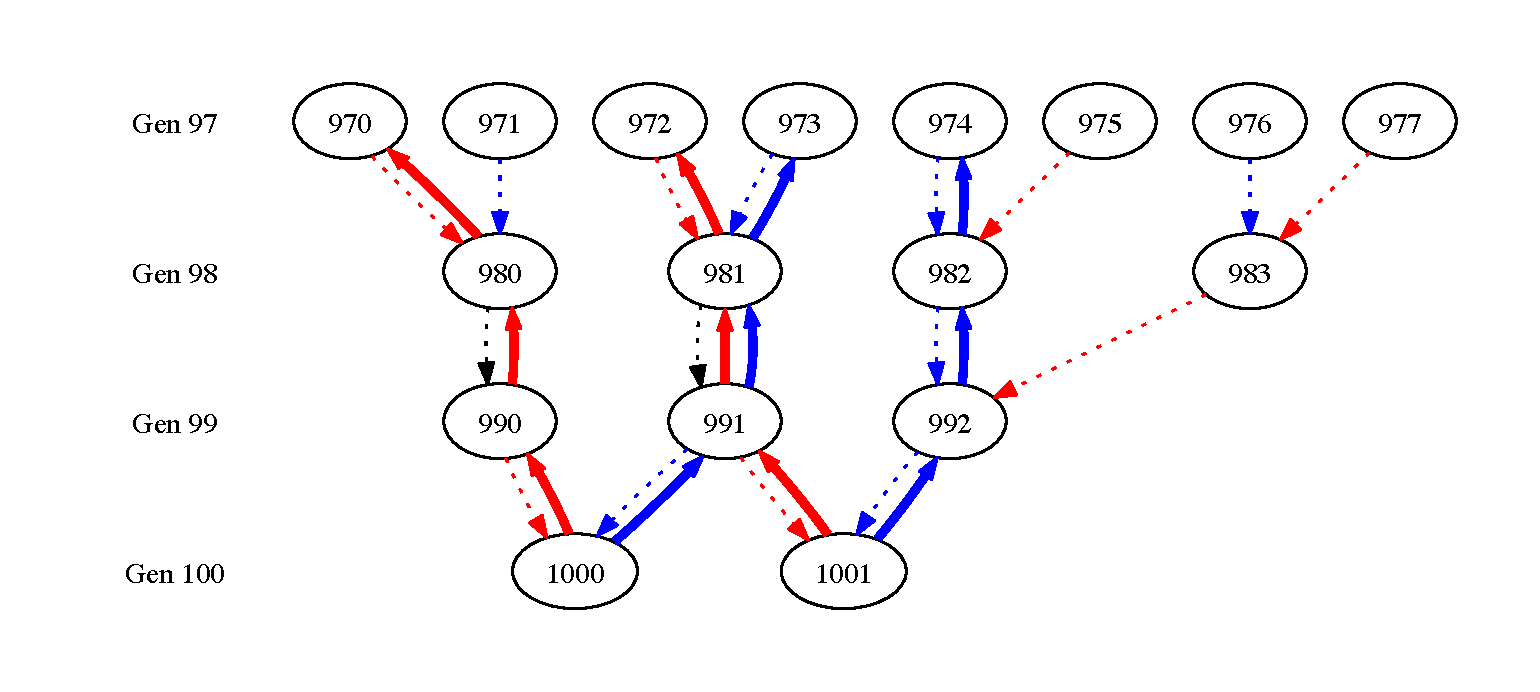
\includegraphics[width=.95\textwidth]{XO_path_example.pdf}
\end{frame}

\subsection{Symbolic Regression and Fitness}

\begin{frame}
	\frametitle{Symbolic Regression and Fitness}
	
	We are focusing on symbolic regression problems.
	\begin{itemize}
		\item Measured data fitted to mathematical formula.
		\item Collection of test points to evolve individuals.
	\end{itemize}
	
	\linespace
	
	Fitness determines individual's distance from target function.
	\begin{itemize}
		\item Lower the fitness, the better the individual.
		\item A zero fitness would exactly match test data.
		\item Anything else to add??????????
	\end{itemize}
	
	\linespace 
	
	The goal of GP is to evolve an individual with a fitness as low as possible.
	
\end{frame}

\section[Graph DB]{Graph Database}
\subsection{Neo4j}

\begin{frame}
	\frametitle{Neo4j}
	
	Neo4j is a graph database.
		\begin{itemize}
		\item Relatively new tool (initial release 2007 popularized in 2010).
		\item Information is stored like a graph.
		\item Nodes and relationships.
		\item Efficient recursive queries.
		\end{itemize}

\end{frame}

\subsection{Cypher}

\begin{frame}
	\frametitle{Cypher}
	Neo4j's query language is Cypher.
	\begin{columns}
	\begin{column}{0.40\textwidth}

	Fundamental elements of Cypher queries:
		\begin{itemize}
		\item START
		\item RETURN
		\item MATCH
		\item WHERE
		\end{itemize}
	\end{column}
	\begin{column}{0.60\textwidth}

	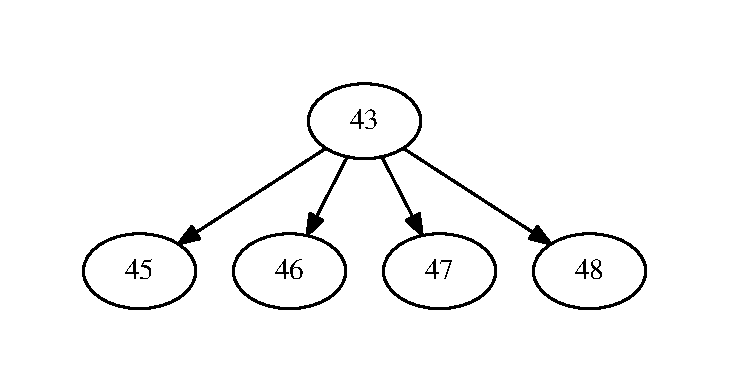
\includegraphics[width=.95\textwidth]{parents.pdf}
	\linebreak
	\emph{
START parent=node(43)
\linebreak
MATCH (parent)-[:PARENTOF]->(child)
\linebreak
RETURN parent, child;
}

	\end{column}	
	\end{columns}
\end{frame}

\section[Setup]{Experimental Setup}

\subsection{Configurations}

\begin{frame}
\frametitle{Run Configurations}
\begin{itemize}
\item[Target Function] sin(x)
\item[Variables] x (range from 0.0 to 6.2, incremented by steps of 0.1)
\item[Constants] range between -5.0 and 5.0
\item[Operations] addition (+), subtraction (-), multiplication (*), protected division (/)
\item[Generation Number] 100
\item[Population Size Per Generation] 1000 (6 runs) and 10000 (1 run)
\item[Transformation Percentages] Crossover (90\%), Mutation (1\%), Reproduction (9\%)
\item[Elitism] best 1\%
\end{itemize}
\end{frame}

\subsection{Methods}

\begin{frame}
\frametitle{Methods}
\begin{itemize}
\item[Fitness] Absolute error between target function and individual function.
\item[PTC2] Randomly adds operators to array of specified length (empty slots for arguments where appropriate). Empty slots divided between variables (63\%) and constants (37\%).
\item[Mutation Type] Subtree Mutation
\end{itemize}
\end{frame}

\section[Results]{Results}

\subsection[Questions Asked]{Questions Asked}

\begin{frame}
\frametitle{Questions Asked}
\begin{enumerate}
\item \emph{How often do mutations improve fitness? Also, how often do crossovers improve fitness, where the root parent is more fit than the non-root parent, and vice versa?}
\item \emph{What does the fitness of the ``winning'' root parent ancestry line look like over time?}
\item \emph{Do a group of individuals have a common root parent ancestor and what is the latest generation where such an ancestor occurs?}
\item \emph{How many individuals in the initial generation have any root parent descendants in the final generation?}
\end{enumerate}
\end{frame}

\subsection[Improved Transformations]{Improved Transformations}

\begin{frame}
\frametitle{Percentage of Improved Transformations}
\emph{How often do mutations and crossovers improve fitness?}
\begin{columns}
\begin{column}{0.5\textwidth}
\begin{center}
{\tiny Results for 10000 Individual Run}
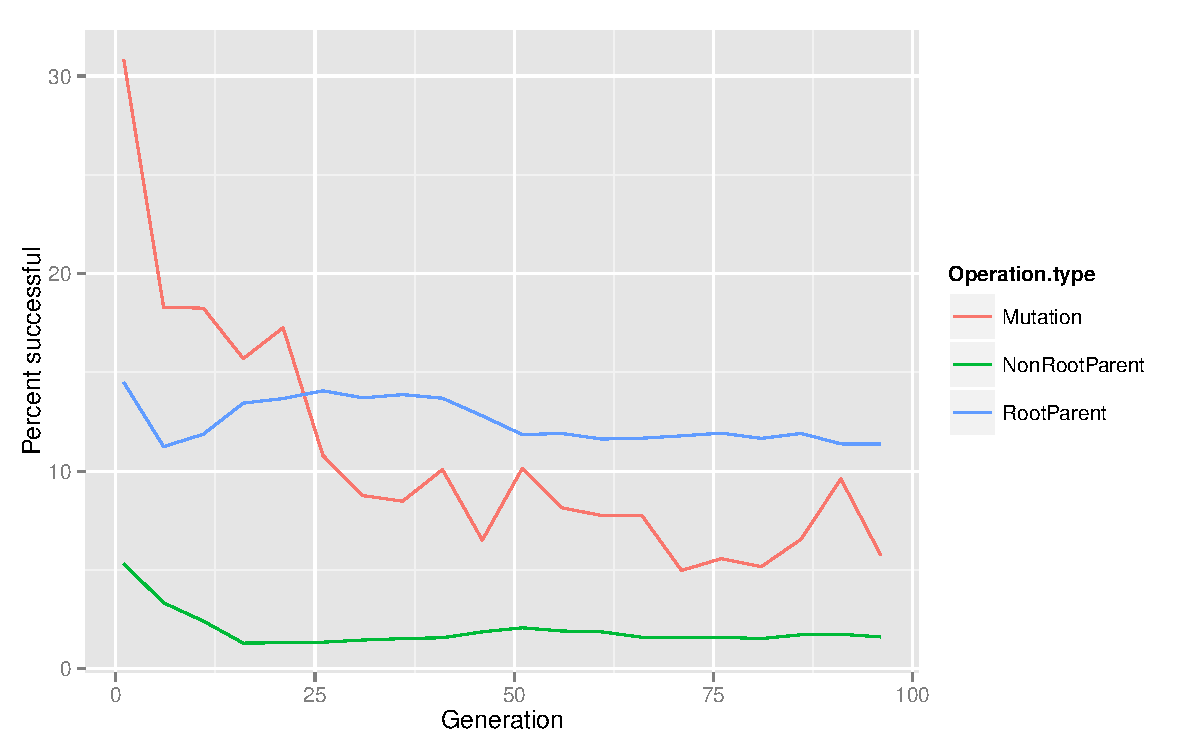
\includegraphics[width=0.95\textwidth]{Blocked_success_percentages}
\end{center}
\end{column}
\begin{column}{0.5\textwidth}
\begin{center}
{\tiny Results for Three 1000 Individual Runs}
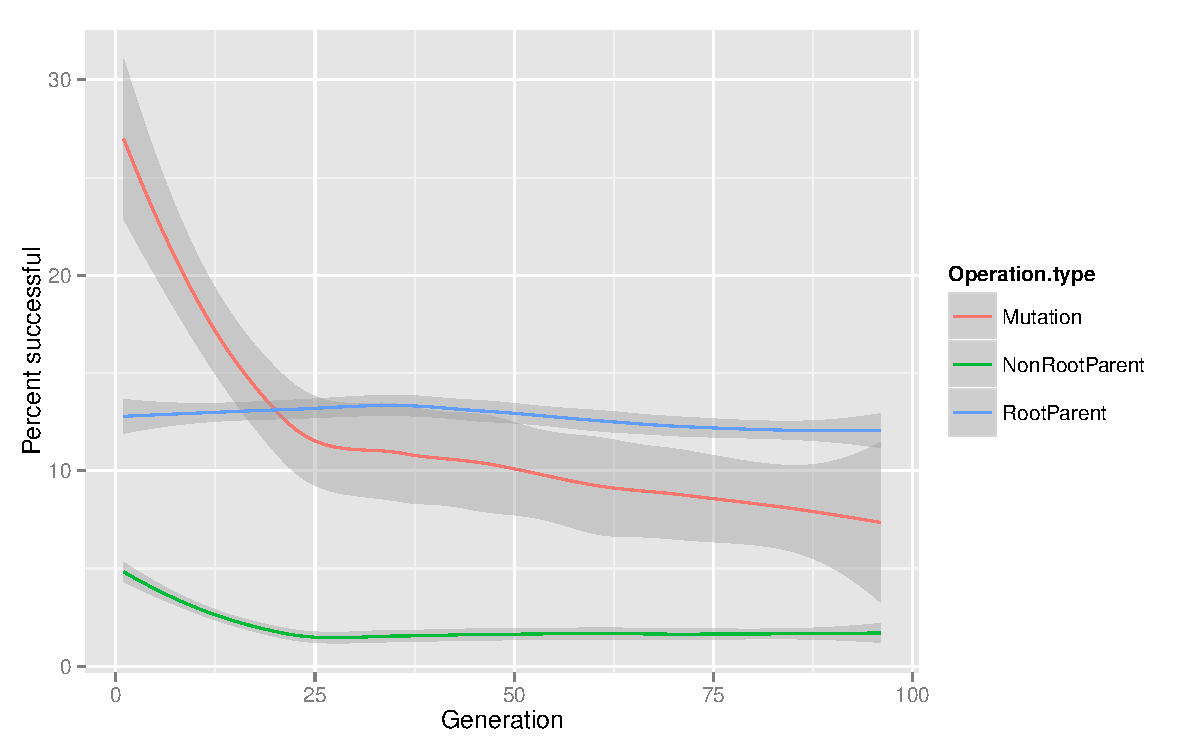
\includegraphics[width=0.95\textwidth]{Percent_successful_Axiom_1K_runs}
\end{center}
\end{column}
\end{columns}
\end{frame}

\subsection[Fitness Graph]{Fitness Over Time}

\begin{frame}
\frametitle{Fitness Over Time}
\emph{What does the fitness of the ``winning'' root parent ancestry line look like over time?}
\begin{center}
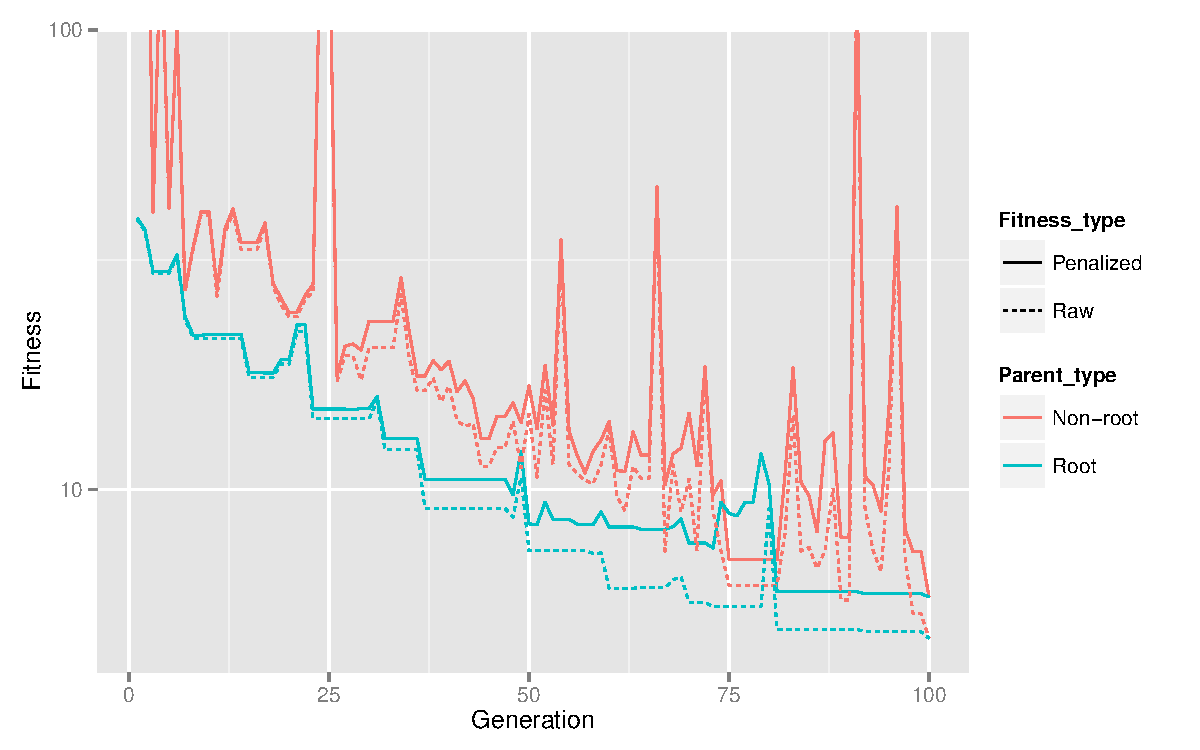
\includegraphics[width=0.85\textwidth]{Combined_fitness_over_time}
\end{center}
\end{frame}

\subsection[Common Ancestor]{Common Ancestor}

\begin{frame}
\frametitle{Common Ancestor}
\emph{Do a group of individuals have a common root parent ancestor and what is the latest generation where such an ancestor occurs?}
\begin{center}
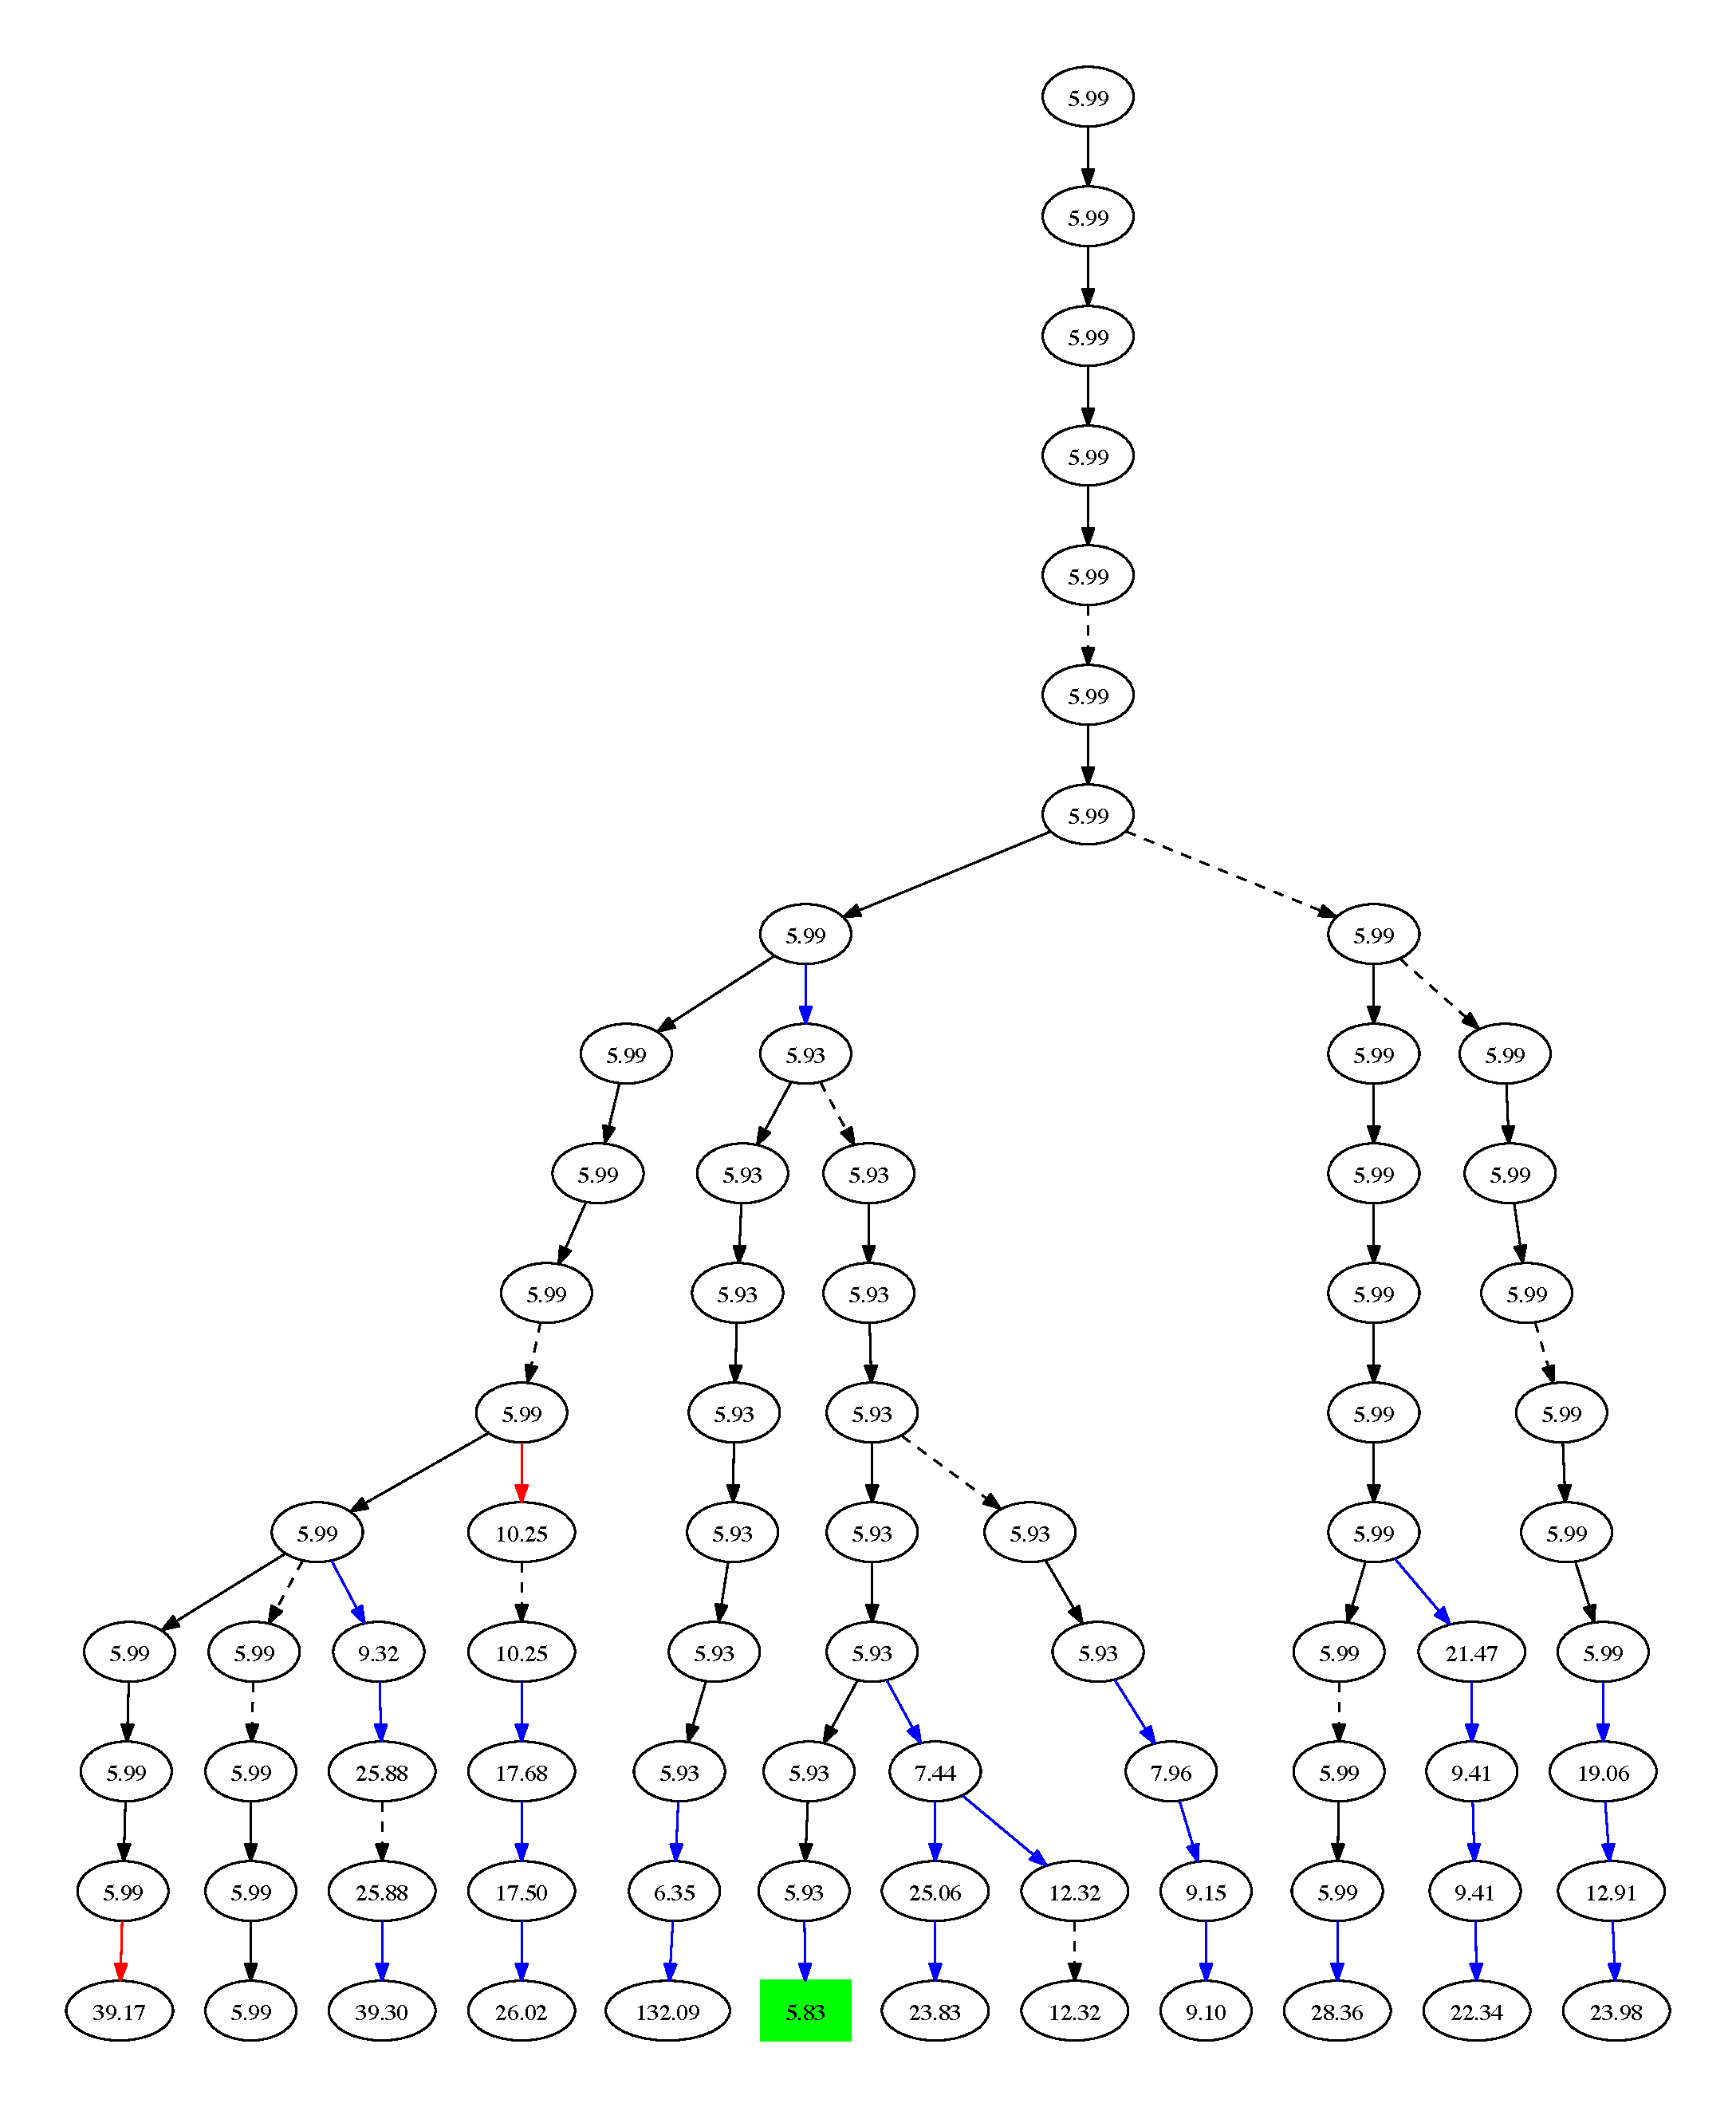
\includegraphics[height=0.75\textheight]{subset_confluence_trimmed}
\end{center}

\end{frame}

\section[Conclusions]{Conclusions}

\begin{frame}
\frametitle{Conclusions}

\begin{itemize}
\item We can gather internal data!
\item Provides more in depth information than statistical summaries. 
\item Support for hypotheses.
\end{itemize}
\linespace
\linespace
\linespace
\linespace

Future work
\begin{itemize}
\item Trying different setup configurations.
\item Enforcing the root parent to have better fitness in XO.
\item Dynamically change parameters.
\end{itemize}
\end{frame}

\begin{frame}
	\frametitle{Thanks!}
	
	Thank you for your time and attention!
		
	\linespace
	\linespace
	
	Contacts:  
	\begin{itemize}
		\item \texttt{donat056@morris.umn.edu}
		\item \texttt{dramd002@morris.umn.edu}
		\item \texttt{mcphee@morris.umn.edu}
	\end{itemize}
	
	\linespace
	\linespace
	
	\begin{center}
	{\huge Questions?}
	\end{center}
\end{frame}

\section*{References}

\begin{frame} 
	\frametitle{References} 
	
	\begin{thebibliography}{lskdjf}
	
	\bibitem{McPhee:2009:gecco}
N.~F. McPhee, E.~Crane, S.~Lahr, and R.~Poli.
\newblock Developmental Plasticity in Linear Genetic Programming.
\newblock In G\"unther Raidl, \emph{et al}, editors, {\em GECCO '09}, pages 1019--1026, Montr\'eal, Qu\'ebec, Canada, 2009.
	
	\bibitem{citeulike:3452411}
	R.~Poli and N.~McPhee.
\newblock A linear estimation-of-distribution {GP} system.
\newblock In M.~O'Neill, \emph{et al}, editors, {\em EuroGP 2008}, volume
  4971 of {\em LNCS}, pages 206--217, Naples,
  26-28 Mar. 2008. Springer.
  
  	\end{thebibliography}
	
	\linespace
	\begin{center}
	See the GECCO '09 paper for additional references.
	\end{center}
\end{frame} 

\end{document}


